\chapter{Java Grundlagen}
\renewcommand{\chaptertitle}{Java Grundlagen}

\lehead[]{\sf\hspace*{-2.00cm}\textcolor{white}{\colorbox{lightblue}{\makebox[1.60cm][r]{\thechapter}}}\hspace{0.17cm}\textcolor{lightblue}{\chaptertitle}}
\rohead[]{\textcolor{lightblue}{\chaptertitle}\sf\hspace*{0.17cm}\textcolor{white}{\colorbox{lightblue}{\makebox[1.60cm][l]{\thechapter}}}\hspace{-2.00cm}}
%\chead[]{}
\rehead[]{\textcolor{lightblue}{AvHG, Inf, My}}
\lohead[]{\textcolor{lightblue}{AvHG, Inf, My}}

\lstset{style=myJava}


\section{Wichtige Regeln}

\begin{compactitem}
\item Es wird zwischen Groß- und Kleinschreibung unterschieden!

\item Alle Anweisungen müssen mit einem Semikolon beendet werden!

\item Mehrere Anweisungen können zu einem Anweisungsblock zusammengefasst
werden. Der Beginn eines Anweisungsblocks wird durch \lstinline|{| und das Ende
durch \lstinline|}| gekennzeichnet.

\item Prozeduren (tun etwas, liefern aber kein Ergebnis) und Funktionen (tun
etwas und geben ein Ergebnis als Rückgabewert zurück) werden in Java als
\emph{Methoden} bezeichnet. Methoden erkennt man immer an den runden Klammern
nach dem Namen. In diesen Klammern steht entweder nichts oder die Parameter, die
von der Methode verarbeitet werden.

Beispiele: \lstinline|close()|, \lstinline|compare(a, b)|

\item In Java ist es üblich, die Namen von Variablen und Methoden mit einem
kleinen Anfangsbuchstaben zu beginnen (auch wenn der Deutschlehrer das nicht
gut findet, der sieht euren Code nicht!).

Beispiele: \lstinline|auto|, \lstinline|zeichneAuto()|

\item In Java ist jedes Programm eine \emph{Klasse}. Was das genau bedeutet,
werden wir uns später ansehen. Alle Variablen und Methoden müssen innerhalb der
geschweiften Klammern der Klasse stehen. Der Name der Datei muss immer genau so
heißen wie der Name der Klasse. Namen von Klassen beginnen üblicherweise mit
einem Großbuchstaben, z.B. \myClass{Auto}, \myClass{MeinProgramm}.
\end{compactitem}


\section{Variablen}

\subsection{Deklaration und Initialisierung}

Die \emph{Deklaration} (Vereinbarung) einer Variablen hat die Form:

\lstinline|Typname Variablenname;|

Beispiel:

\begin{lstlisting}
int i, j;
double zahl;
\end{lstlisting}


Bei der Deklaration darf die Variable auch gleichzeitig \emph{initialisiert}
werden.
Das bedeutet, dass sie einen Anfangswert erhält. Beispiel:

\begin{lstlisting}
int i = 45, j = 3;
double zahl = 0.0;
\end{lstlisting}

\subsection{Lebensdauer}

Die Lebensdauer einer lokalen Variablen, die innerhalb einer Methode deklariert
wird, erstreckt sich von der Stelle ihrer Deklaration bis zum Ende der Methode.
Falls eine Variable innerhalb eines geklammerten Blocks deklariert wird, lebt
die Variable nur bis zum Ende des Blocks.

Globale Variablen, die außerhalb einer Methode stehen, gehören immer zu einer
Klasse und müssen innerhalb der Klasse stehen.

\subsection{Konstanten}

Einer Variable, deren Wert nicht verändert werden soll, wird das Schlüsselwort
\lstinline|final| vorangestellt. Damit wird die Variable zu einer
\emph{Konstanten}. Die Namen von Konstanten werden üblicherweise komplett groß
geschrieben. Beispiel:

\begin{lstlisting}
final float PI = 3.14;
final String NAME = "Otto Mustermann";
\end{lstlisting}


\section{Kommentare}

\begin{lstlisting}
int i, j; æ// Kommentar bis zum Zeilenende

/* Kommentar über
 * mehrere Zeilen
 */æ
\end{lstlisting}


\section{Namenskonventionen}

Zur besseren Lesbarkeit des Codes gibt es folgende Konventionen:

\begin{tabular}{|l|l|l|l|}\hline
\textbf{Art} & \textbf{Namensgebung} & \textbf{Schreibweise} & \textbf{Beispiel}
\\ \hline
Klasse & Substantiv (Einzahl) & CamelCase mit großem Anfangsbuchstaben &
{\lstinline|String|}, {\lstinline|Auto|} \\ \hline
Variable, Objekt &  & camelCase mit
kleinem Anfangsbuchstaben & {\lstinline|meinAuto|} 
\\ \hline
Methode & Verb & camelCase mit kleinem
Anfangsbuchstaben & {\lstinline|zeichneAuto()|}
\\ \hline
Konstante & & komplett mit Großbuchstaben &
{\lstinline|WIDTH|} 
\\
&& verbunden mit Unterstrichen &  {\lstinline|MIN_HEIGHT|}
\\ \hline
\end{tabular}

Alle Namen müssen immer mit einem Buchstaben beginnen und dürfen keine
Leerzeichen enthalten. 

Außerdem gilt als Grundregel: Bezeichner sollten möglichst kurz und \glqq
sprechend\grqq (selbsterklärend) sein. Ausgenommen von dieser Regel sind
Variablen, die nur kurzzeitig (etwa als Zähler innerhalb einer Schleife) benutzt
werden. Solche \glqq Wegwerfvariablen\grqq werden oft wie folgt benannt:

\lstinline|i|, \lstinline|j|, \lstinline|k|, \lstinline|m|, und \lstinline|n|
für Ganzahl-,  \lstinline|x|, \lstinline|y|, und \lstinline|z| für
Fließkomma- und schließlich \lstinline|c|, \lstinline|d|, und
\lstinline|e| für Character-Variablen.

Siehe auch
\url{http://www.oracle.com/technetwork/java/codeconventions-135099.html}


\section{Datentypen}

Folgende Datentypen stehen zur Verfügung:

\begin{savenotes}
\begin{tabular}{|l|l|c|l|l|}\hline
\textbf{Datentyp} & \textbf{Bedeutung} & \textbf{Anzahl Bytes} &
\textbf{Wertebereich} & \textbf{Standardwert}
\\ \hline
{\lstinline|boolean|} & Wahrheitswerte & 1 & {\lstinline|true|},
{\lstinline|false|} & {\lstinline|false|} 
\\ \hline
{\lstinline|char|} & Buchstaben & 2 & Alle Unicode-Zeichen &
{\lstinline|\u0000|} 
\\
&&(Fußnote\footnote{Einige seltene Unicode-Zeichen werden als eine Folge von
zwei \texttt{char}-Objekten verpackt.\\ Siehe
\url{http://docs.oracle.com/javase/tutorial/i18n/text/unicode.html}})&&
\\
\hline {\lstinline|byte|} & ein Byte große Zahlen & 1 & -128 ... 127 & 0 
\\ \hline
{\lstinline|short|} & kleine ganze Zahlen & 2 & $-2^{7} ... 2^{7}-1$
(-32.768...32.767) & 0 \\ \hline
{\lstinline|int|} & ganze Zahlen & 4 & $-2^{31} ... 2^{31}-1$ & 0 
\\ \hline 
{\lstinline|long|} & große ganze Zahlen & 8 & $-2^{63} ... 2^{63}-1$ & 0
\\ \hline
{\lstinline|float|} & kleine Fließkommazahlen & 4 & $\pm 3.40282347 \cdot
10^{38}$ & 0.0 \\ 
&&& (Fußnote\footnote{Tatsächlich ist der Wertebereich von \texttt{float} und
\texttt{double} im negativen sogar noch größer als im positiven.\\ Siehe
\url{http://de.wikibooks.org/wiki/Java_Standard:_Primitive_Datentypen}})&
\\
\hline {\lstinline|double|} & große Fließkommazahlen & 8 & $\pm 1.79769313486231570
\cdot 10^{308}$ & 0.0
\\ \hline
{\lstinline|String|} & Zeichenketten & & & leerer String
\\ \hline
\end{tabular}
\end{savenotes}

Neben den Standard-Datentypen kann man sich eigene Datentypen definieren, in dem
man eine eigene Klasse schreibt. Der Typ \myClass{String} ist eine vordefinierte
Klasse aus dem Package \myPackage{java.lang}.


\section{Typkonvertierungen}

Zwischen den primitiven Datentypen besteht die folgende Beziehung:

\begin{center}
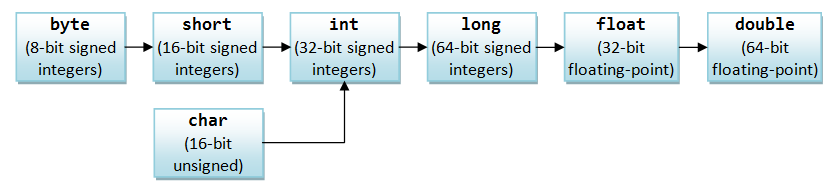
\includegraphics[width=0.9\textwidth]{./inf/SEKII/04_Java_Grundlagen/JavaBasics_ImplicitTypeCastingPrimitives.png}
% Quelle: http://www.ntu.edu.sg/home/ehchua/programming/java/J2_Basics.html
% erlaubnis zur verwendung per e-mail von ehchua@ntu.edu.sg vom 5.8.13:
% --- snip -----
% You can use for teaching in public schools, but not for commercial purposes.
% Hock Chuan
% --- snap -----
\end{center}

Die Konvertierung eines „kleineren“ in einen „größeren“ Datentyp (also von links
nach rechts im Schaubild) führt das System automatisch durch. Eine Konvertierung
in umgekehrter Richtung kann einen Datenverlust bedeuten und wird deshalb nur
auf explizite Anweisung des Programmierers vorgenommen. Beispiel:

\begin{lstlisting}
int i = 56;
double d = 24.5;
double d2 = i;      æ// geht automatisch
æint i2 = (int) d;   æ// explizite Typkonvertierung, vom Programmierer erzwungen
æchar c = (char) i;  æ// explizite Typkonvertierung
\end{lstlisting}

Das Schema einer expliziten Typkonvertierung lautet:

\verb|Variable_vom_Typ1 = (Typ1) Variable_vom_Typ2;|

Andere Konvertierungen (z.B. zwischen int und String) können nur mit Hilfe
spezieller Methoden durchgeführt werden. Zahlenvariablen werden jedoch
automatisch in einen String umgewandelt, wenn man sie mit einem ’\lstinline|+|’
an einen String anhängt. Beispiel:

\begin{lstlisting}
String text = "Der Inhalt von i ist: " + i;
\end{lstlisting}


\section{Literale}

\begin{description}
\item{\textbf{Ganzzahlige Zahlenwerte}} (z.B. \lstinline|304|) sind
grundsätzlich vom Typ \lstinline|int|. Nur wenn der Suffix \lstinline|l| oder \lstinline|L| hinten
angehängt wird (z.B. \lstinline|304L|) sind sie vom Typ \lstinline|long|.

\item{\textbf{Zahlenwerte von Fließkommazahlen}} enthalten im Gegensatz zu
ganzen Zahlen einen Punkt zur Trennung der Nachkommastelle (z.B. ist \lstinline|0| eine ganze Zahl
aber \lstinline|0.0| ist eine Fließkommazahl). Standardmäßig sind
Fließkommazahlen vom Typ \lstinline|double|. Wenn man eine Fließkommazahl vom
Typ \lstinline|float| haben möchte, muss man das Suffix \lstinline|f| oder
\lstinline|F| an die Zahl anhängen (z.B. \lstinline|0.0F|).

Für Fließkommazahlen sind einige symbolische Zahlenwerte verfügbar:

\begin{tabular}{|l|l|}\hline
\textbf{Name} & \textbf{Bedeutung} \\ \hline
{\lstinline|MAX_VALUE|} & Größter darstellbarer positiver Wert \\ \hline
{\lstinline|MIN_VALUE|} & Kleinster darstellbarer positiver Wert \\ \hline
{\lstinline|NaN|} & Not-A-Number \\ \hline
{\lstinline|NEGATIVE_INFINITY|} & Negativ unendlich \\ \hline
{\lstinline|POSITIVE_INFINITY|} & Positiv unendlich \\ \hline
\end{tabular}

\item{\textbf{Buchstaben (\lstinline|char|)}} werden grundsätzlich in einfache
Hochkommata gesetzt.

\item{\textbf{Zeichenketten (\lstinline|String|)}} werden mit doppelten
Hochkommata geschrieben. Zur Darstellung von Sonderzeichen gibt es eine Reihe
von Standard-Escape-Sequenzen:

\begin{tabular}{|l|l|}\hline
\textbf{Zeichen} & \textbf{Bedeutung} \\ \hline
{\lstinline|\b|} & Rückschritt (Backspace) \\ \hline
{\lstinline|\t|} & Horizontaler Tabulator \\ \hline
{\lstinline|\n|} & Zeilenschaltung (Newline) \\ \hline
{\lstinline|\f|} & Seitenumbruch (Formfeed) \\ \hline
{\lstinline|\r|} & Wagenrücklauf (Carriage return) \\ \hline
{\lstinline|\"|} & Doppeltes Anführungszeichen \\ \hline
{\lstinline|\'|} & Einfaches Anführungszeichen \\ \hline
{\lstinline|\\|} & Backslash \\ \hline
{\lstinline|\nnn|} & Oktalzahl nnn (kann auch kürzer als 3 Zeichen sein, darf
nicht größer als oktal 377 sein) \\ \hline 
{\lstinline|\uxxxx|} & Unicode-Escape-Sequenz. xxxx steht für eine Folge von 4
hexadezimalen Ziffern.\\
& Z.B. ist {\lstinline|\u0020|} die Hexadezimaldarstellung des Leerzeichens. 
\\ \hline
\end{tabular}

Beispiele:

\begin{lstlisting}
char c = 'a', b = '\t';
String text = "Guten Tag.\nWie geht es dir?";
\end{lstlisting}
\end{description}


\section{Operatoren}

\subsection{Arithmetische Operatoren}

\begin{tabular}{|c|l|l|}\hline
\textbf{Operator} & \textbf{Bezeichnung} & \textbf{Bedeutung}
\\ \hline
{\lstinline|+|} & Addition & {\lstinline|a + b|} ergibt die Summe von
{\lstinline|a|} und {\lstinline|b|}
\\ \hline
{\lstinline|-|} & Subtraktion & {\lstinline|a - b|} ergibt die Differenz von
{\lstinline|a|} und {\lstinline|b|}
\\ \hline
{\lstinline|*|} & Multiplikation & {\lstinline|a * b|} ergibt das Produkt
von {\lstinline|a|} und {\lstinline|b|}
\\ \hline
{\lstinline|/|} & Division & {\lstinline|a / b|} ergibt den Quotienten
von {\lstinline|a|} und {\lstinline|b|}
\\ \hline
%###
{\lstinline|%|} & Modulo (Restwert) & {\lstinline|a % b|} ergibt den Rest der
ganzzahligen Division von {\lstinline|a|} und {\lstinline|b|}
\\ 
%###
& & Lässt sich in Java auch auf Fließkommazahlen anwenden.
\\ \hline
{\lstinline|++|} & Präinkrement & {\lstinline|x = ++a;|} erhöht {\lstinline|a|}
um {\lstinline|1|} und schreibt das Ergebnis ({\lstinline|a+1|}) in
{\lstinline|x|}
\\ \hline
{\lstinline|++|} & Postinkrement & {\lstinline|x = a++;|} schreibt
{\lstinline|a|} in {\lstinline|x|} und erhöht {\lstinline|a|} anschließend um
{\lstinline|1|} 
\\ \hline
{\lstinline|--|} & Prädekrement & {\lstinline|x = --a;|} verringert
{\lstinline|a|} um {\lstinline|1|} und schreibt das Ergebnis ({\lstinline|a-1|})
in {\lstinline|x|} 
\\ \hline
{\lstinline|--|} & Postdekrement & {\lstinline|x = a--;|} schreibt
{\lstinline|a|} in {\lstinline|x|} und verringert {\lstinline|a|} anschließend
um {\lstinline|1|}
\\ \hline
\end{tabular}


\subsection{Vergleichs-Operatoren}

\begin{tabular}{|c|l|l|}\hline
\textbf{Operator} & \textbf{Bezeichnung} & \textbf{Bedeutung}
\\ \hline
{\lstinline|==|} & gleich & {\lstinline|a == b|} ergibt {\lstinline|true|}, wenn
{\lstinline|a|} gleich {\lstinline|b|} ist. Sind {\lstinline|a|} und
{\lstinline|b|} Referenztypen,  so ist\\
&&
der Rückgabewert {\lstinline|true|}, wenn beide Werte auf dasselbe Objekt
zeigen.
\\ \hline
{\lstinline|!=|} & ungleich & {\lstinline|a != b|} ergibt {\lstinline|true|},
wenn {\lstinline|a|} ungleich {\lstinline|b|} ist. Sind {\lstinline|a|} und
{\lstinline|b|} Objekte, so ist der\\
&&  Rückgabewert
{\lstinline|true|}, wenn beide Werte auf unterschiedliche Objekte zeigen.
\\ \hline
{\lstinline|<|} & kleiner & {\lstinline|a < b|} ergibt {\lstinline|true|}, wenn
{\lstinline|a|} kleiner {\lstinline|b|} ist.
\\ \hline
{\lstinline|<=|} & kleiner gleich & {\lstinline|a <= b|} ergibt
{\lstinline|true|}, wenn {\lstinline|a|} kleiner oder gleich {\lstinline|b|}
ist.
\\ \hline
{\lstinline|>|} & größer & {\lstinline|a > b|} ergibt {\lstinline|true|}, wenn
{\lstinline|a|} größer {\lstinline|b|} ist.
\\ \hline
{\lstinline|>=|} & größer gleich & {\lstinline|a >= b|} ergibt
{\lstinline|true|}, wenn {\lstinline|a|} größer oder gleich {\lstinline|b|}
ist.
\\ \hline
\end{tabular}


\subsection{Logische Operatoren}

\begin{tabular}{|c|l|l|}\hline
\textbf{Operator} & \textbf{Bezeichnung} & \textbf{Bedeutung}
\\ \hline
{\lstinline|!|} & logisches NICHT & {\lstinline|!a|} ergibt {\lstinline|false|},
wenn {\lstinline|a|} wahr ist, und {\lstinline|true|}, wenn {\lstinline|a|}
falsch ist.
\\ \hline
{\lstinline|&&|} & UND mit Short- &
{\lstinline|a && b|} ergibt {\lstinline|true|}, wenn sowohl {\lstinline|a|} als
auch {\lstinline|b|} wahr sind. Ist {\lstinline|a|} bereits\\
& Cirquit-Evaluation & falsch, so wird
{\lstinline|false|} zurückgegeben und {\lstinline|b|} nicht mehr ausgewertet.
\\ \hline
{\lstinline!||!} & ODER mit Short- &
{\lstinline!a || b!} ergibt {\lstinline!true!}, wenn mindestens einer der beiden
Ausdrücke {\lstinline!a!}\\
& Circuit-Evaluation & oder {\lstinline!b!} wahr ist. Ist bereits
{\lstinline!a!} wahr, so wird {\lstinline!true!} zurückgegeben und
{\lstinline!b!}\\
&& nicht mehr ausgewertet.
\\ \hline
{\lstinline!&!} & UND ohne Short- &
{\lstinline!a & b!} ergibt {\lstinline!true!}, wenn sowohl {\lstinline!a!} als
auch {\lstinline!b!} wahr sind.\\
{} & Circuit-Evaluation & Beide Teilausdrücke werden ausgewertet.
\\ \hline
{\lstinline!|!} &  ODER ohne Short- &
{\lstinline!a | b!} ergibt {\lstinline!true!}, wenn mindestens einer der beiden
Ausdrücke\\
& Circuit-Evaluation & {\lstinline!a!} oder {\lstinline!b!} wahr ist. Beide
Teilausdrücke werden ausgewertet.
\\ \hline
{\lstinline!^!} & Exklusiv-ODER & {\lstinline!a ^ b!} ergibt {\lstinline!true!},
wenn beide Ausdrücke einen unterschiedlichen\\
&& Wahrheitswert haben.
\\ \hline
\end{tabular}


\subsection{Zuweisungsoperatoren}

\begin{tabular}{|c|l|l|}\hline
\textbf{Operator} & \textbf{Bezeichnung} & \textbf{Bedeutung}
\\ \hline
{\lstinline|=|} & einfache Zuweisung & {\lstinline|a = b;|} weist
{\lstinline|a|} den Wert von {\lstinline|b|} zu und liefert {\lstinline|b|} als
Rückgabewert.
\\ \hline
{\lstinline|+=|} & Additionszuweisung & {\lstinline|a += b;|} ist eine Abkürzung
für {\lstinline|a = a + b;|}
\\ \hline
{\lstinline|-=|} & Subtraktionszuweisung & {\lstinline|a -= b;|} ist eine
Abkürzung für {\lstinline|a = a - b;|} 
\\ \hline
{\lstinline|*=|} & Multiplikationszuweisung & {\lstinline|a *= b;|} ist
eine Abkürzung für {\lstinline|a = a * b;|}
\\ \hline
{\lstinline|/=|} & Divisionszuweisung & {\lstinline|a /= b;|} ist
eine Abkürzung für {\lstinline|a = a / b;|}
\\ \hline
%###
{\lstinline|%=|} & Modulozuweisung & {\lstinline|a %= b;|} ist eine Abkürzung
für {\lstinline|a = a % b;|}
\\ \hline
%###
\end{tabular}


\section{Kontrollstrukturen}

\subsection{Einfache Verzweigung}

\begin{lstlisting}
if (`\slshape{Bedingung}`) {
  `\slshape{Anweisungen}`;
}
else {
  `\slshape{Anweisungen}`;
}
\end{lstlisting}

Der \lstinline|else|-Teil kann auch entfallen. Die Klammern dürfen weggelassen
werden, wenn es nur eine einzige Anweisungszeile gibt.


\subsection{Mehrfach-Verzweigung}

\begin{lstlisting}
switch (`\slshape{Ausdruck}`) {
case `\slshape{Wert1}`:
  `\slshape{Anweisungen1}`;
  break;           æ// Achtung: ohne break; wird auch Anweisungen2 ausgeführt!
æcase `\slshape{Wert2}`:
  Anweisungen2;
  break;
...
default:           æ// falls kein anderer Wert passt (optional)
æ  `\slshape{Anweisungen3}`;
}
\end{lstlisting}

\pagebreak

Beispiel:

\begin{lstlisting}
switch (ampelfarbe) {
case "rot":
case "gelb": 
  warten();
  break;
case "grün":
  gehen();  
  break;
default:
  System.out.println("Das ist aber eine komische Ampel!");
}
\end{lstlisting}


\subsection{Schleifen}

\begin{compactenum}[a)]
\item
\begin{lstlisting}
while (`\slshape{Bedingung}`) {
  `\slshape{Anweisungen}`;
}
\end{lstlisting}

Beispiel:

\begin{lstlisting}
int zaehler = 0;
while (zaehler<10) {
  System.out.println("Der Zähler hat den Wert: " + zaehler);
  zaehler++;     æ// Kurzform für: zaehler = zaehler + 1;
æ}
\end{lstlisting}

Die Anweisungen in den geschweiften Klammern werden ausgeführt, solange die
Bedingung \lstinline|true| ergibt.

\item 
\begin{lstlisting}
do {
  `\slshape{Anweisungen}`;
} while (`\slshape{Bedingung}`);
\end{lstlisting}


Die Anweisungen in den geschweiften Klammern werden ausgeführt, solange die
Bedingung \lstinline|true| ergibt (mindestens aber ein mal).

\item
\begin{lstlisting}
for (`\slshape{Vorab}`; `\slshape{Bedingung}`; `\slshape{Wert-Verändern}`) {
  `\slshape{Anweisungen}`;
}
\end{lstlisting}

Der Teil \emph{Vorab} wird nur einmal ausgeführt, bevor die Schleife
betreten wird. Hier fügt man den Code zur Initialisierung der Variable ein. Die
Schleife wird ausgeführt, solang die \emph{Bedingung} wahr ist. Nach
jedem Schleifendurchgang wird der Code \emph{Wert-Verändern} einmal
ausgeführt. Das obige Beispiel für die \lstinline|while|-Schleife kann man mit
der \lstinline|for|-Schleife folgendermaßen schreiben:

\begin{lstlisting}
for (int zaehler = 0; zaehler < 10; zaehler++) {
  System.out.println ("Der Zähler hat den Wert: " + zaehler);
}
\end{lstlisting}
\end{compactenum}


\section{Methoden}

Aufgaben die mehrere Anweisungen umfassen und die immer wieder, auch an
verschiedenen Stellen des Programms ausgeführt werden sollen, kann man in
\emph{Methoden} \glqq verpacken\grqq :

Methoden müssen immer innerhalb einer Klasse stehen. Eine Methode hat
folgendes Schema:

\begin{lstlisting}
`\slshape{Sichtbarkeit Rückgabewert Name}`(`\slshape{Typ1 Parameter1}`, `\slshape{Typ2 Parameter2}`, ...) { 
  `\slshape{Anweisungen}`; 
  return `\slshape{Wert}`;         æ// Rückgabe eines berechneten Wertes. Kann entfallen.
æ}
\end{lstlisting}

Die \emph{Sichtbarkeit} regelt, wer das Recht hat, die Methode aufzurufen. Der
Wert \lstinline|public| gibt z.B. an, dass die Methode öffentlich ist und jeder
darauf zugreifen kann.

Der \emph{Rückgabewert} gibt an, welchen Typ die Werte haben, die die Methode
zurück liefert. Wenn die Methode keinen Wert zurück liefert, schreibt man
\lstinline|void|. Wenn die Methode einen Wert zurück gibt, gibt man an dieser
Stelle den Typ des Werts an.

Standard-Datentypen (\lstinline|int|, \lstinline|boolean|, usw.) können in Java
nur als Werte-Parameter übergeben werden, d.h.
es wird eine Kopie einer Variablen übergeben. Objekt-Variablen sind dagegen
immer Referenz-Parameter, d.h. die Speicheradresse der Objekte wird übergeben.

Beispiele:

\begin{lstlisting}
public void schreibeText() {
  System.out.println ("Hallo");         æ// schreibt Text auf die Konsole
æ}

public int mult(int zahl1, int zahl2) {
  int ergebnis = zahl1 * zahl2;
  return ergebnis;
}
\end{lstlisting}

Der Aufruf der obigen Methoden von einer anderen Methode innerhalb derselben Klasse kann z.B.
folgendermaßen aussehen:

\begin{lstlisting}
schreibeText();                         æ// die Klammern dürfen nicht fehlen!
æint zahl = mult(5, 4);
\end{lstlisting}